\section*{Appendix A}
\lstset{
 upquote=true,
 showspaces=false,
 showtabs=false,
 frame=none,
 tabsize=2,
 breaklines=true,
 numbers=none,
 showstringspaces=false,
 breakatwhitespace=true,
 escapeinside={(*@}{@*)},
 keywordstyle=\bfseries,
 basicstyle=\scriptsize\ttfamily,
 moredelim=**[is][\color{red}]{@}{@},
}

In this appendix are reported the answers to the questions proposed in all the
previous lab activities.


\subsection*{Activity 1}

\subsubsection*{Task 7 - Step 2}
\textit{Test the created topology: verify the network connectivity between all hosts.
Write in the lines below the commands you used and the results you obtained.}
\begin{figure}[htb]
	\centering
	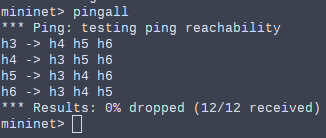
\includegraphics[width=0.5\linewidth]{img/task-7-step-2.png}
\end{figure}



\subsubsection*{Task 7 - Step 3}
\textit{Verify that the bandwidth and the delay of each link comply with the values
specified in the topology diagram shown in figure 1. Write in the lines below
the commands you used and the results you obtained.}

\begin{itemize}
  \item \code{h3 ping h4 -c 10}

  Output:
  \begin{lstlisting}
  --- 10.0.0.2 ping statistics ---
  5 packets transmitted, 5 received, 0% packet loss, time 4006ms
  rtt min/avg/max/mdev = 23.186/25.264/26.760/1.507 ms
  \end{lstlisting}
  The average RTT is approximately 20ms, wich complies the link delays values
  specified in the topology diagram. The same proceeding can be used to test the
  delay of all the others links.

  It's important to point out that the link delay between the two switches doesn't
  comply with the topology diagram: this behavior is however acceptable and it's due to
  the fact that in Mininet the switches are by default run in the same network
  namespace inside the kernel space, therefore they communicate to each other
  without using the link which has the performance parameters specified
  in the Python script.

  \item \code{iperf h3 h4}

  Output:
  \begin{lstlisting}
  *** Iperf: testing TCP bandwidth between h3 and h6
  *** Results: ['4.75 Mbits/sec', '6.23 Mbits/sec']
  \end{lstlisting}

  The same proceeding can be used to test the bandwidth between all nodes.
\end{itemize}



\subsubsection*{Task 8 - Question 1}
\textit{What are the advantages of having more controllers instead of
one single controller which serves all the switches of the network?}
\begin{itemize}
  \item \textbf{More performance}:  having more controllers makes each controller serve fewer
  nodes, therefore reducing its workload and improving the network performance.
  Moreover using more controllers makes it possible to choose where to position
  each controller: choosing a good placement increases the performance
  of the newtork by reducing the delay between each switch and the relative
  controller.
  \item \textbf{More fault tolerance}: the SDN controller is not a SPOF \footnote{SPOF = single point of failure}
  anymore because the network includes more controllers, so if one of the them
  fails the network can still work if there is at least another controller which can replace it.
  This can be achieved for example connecting each switch to multiple controllers
  or connecting the switches to a load balancer which acts like a ``man in the middle'' and
  forwards the requests that receives only to working controllers.
\end{itemize}


\subsubsection*{Task 8 - Question 2}
\textit{Would the fault tolerance of the network shown in figure \ref{fig:topology-1}
change if only one controller (linked to both the switches) was used
instead of two?}

No because in this topology each switch is connected only to a single controller,
therefore a failure of one of the two controllers prevents the network from
working properly, just like in the case of a single controller connected to both switches.





\subsubsection*{Task 8 - Question 3}
\textit{In this activity the topology shown in figure 1 was implemented
assuming that the two controllers were local controllers. How
would you have to change the Python script you created in this
activity in order to use remote controllers instead of local ones?
(Hint: see reference [5])}

The changes that has to be applied to the Python script are marked with the red
colour in the listing below.

\lstset{
 upquote=true,
 showspaces=false,
 showtabs=false,
 frame=single,
 tabsize=2,
 breaklines=true,
 numbers=left,
 showstringspaces=false,
 breakatwhitespace=true,
 escapeinside={(*@}{@*)},
 keywordstyle=\bfseries,
 basicstyle=\scriptsize\ttfamily,
 moredelim=**[is][\color{red}]{@}{@},
}
\begin{minipage}{\linewidth}
\begin{lstlisting}
#!/usr/bin/Python
from mininet.net import Mininet
from mininet.node import Controller, OVSSwitch, @RemoteController@
from mininet.cli import CLI
from mininet.log import setLogLevel, info
from mininet.link import TCLink

def multiControllerNet():
    net = Mininet( controller=Controller, switch=OVSSwitch, link=TCLink )

    info( "*** Creating hosts\n" )
    h1 = net.addHost('h3')
    h2 = net.addHost('h4')
    h3 = net.addHost('h5')
    h4 = net.addHost('h6')

    info( "*** Creating switches\n" )
    s1 = net.addSwitch( 's1' )
    s2 = net.addSwitch( 's2' )

    info( "*** Creating links\n" )
    net.addLink( h1, s1, bw=5, delay='5ms' )
    net.addLink( h2, s1, bw=5, delay='5ms' )
    net.addLink( h3, s2, bw=5, delay='5ms' )
    net.addLink( h4, s2, bw=5, delay='5ms' )
    net.addLink( s1, s2, bw=10, delay='2ms' )

    info( "*** Creating (reference) controllers\n" )
    c0 = net.addController( 'c0', @controller=RemoteController, ip='127.0.0.1'@, port=6633 )
    c1 = net.addController( 'c1', @controller=RemoteController, ip='127.0.0.1'@, port=6634 )

    info( "*** Starting network\n" )
    net.build()
    c0.start()
    c1.start()
    s1.start( [ c0 ] )
    s2.start( [ c1 ] )

    info( "*** Running CLI\n" )
    CLI( net )

    info( "*** Stopping network\n" )
    net.stop()

if __name__ == '__main__':
    setLogLevel( 'info' )
    multiControllerNet()
\end{lstlisting}
\end{minipage}
\lstset{
 upquote=true,
 showspaces=false,
 showtabs=false,
 frame=none,
 tabsize=2,
 breaklines=true,
 numbers=none,
 showstringspaces=false,
 breakatwhitespace=true,
 escapeinside={(*@}{@*)},
 keywordstyle=\bfseries,
 basicstyle=\scriptsize\ttfamily,
 moredelim=**[is][\color{red}]{@}{@},
}

For simplicity it has been assumed that the two remote controllers are running on the same machine on
which Mininet is running, therefore the ip \code{127.0.0.1} has been used (if the
controllers had been on different machines the relative IP should have been used).




\subsubsection*{Task 8 - Question 4}
\textit{How could we improve the fault tolerance of the network shown
in figure 1 making minor changes to the Python script used?}

The easiest way is to connect each switch to both the controllers, so that if
one controller fails the other one can still serve the switches keeping therefore
the network working. It is possible to do that simply modifying the lines 36 and 37 of
the Python script used in activity 1 (shown in listing \ref{lst:activity-1-script})
like this:

\begin{lstlisting}
s1.start( [ c0, c1 ] )
s2.start( [ c0, c1 ] )
\end{lstlisting}







\subsection*{Activity 2}
\subsubsection*{Task 5 - Step 2}
\textit{Test the created topology: verify the network connectivity between all hosts.
Write in the lines below the commands you used and the results you obtained.}
\begin{figure}[htb]
	\centering
	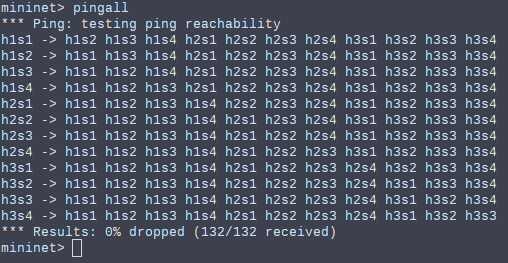
\includegraphics[width=0.8\linewidth]{img/activity-2-task-5-step-2.png}
\end{figure}


\subsubsection*{Task 5 - Step 3}
\textit{Verify the bandwidth and the delay between the hosts h1s1 and h3s4. Write
in the lines below the commands you used and the results you obtained.}
\begin{itemize}
  \item \code{iperf h1s1 h3s4}

  Result:
  \begin{lstlisting}
  *** Iperf: testing TCP bandwidth between h1s1 and h3s4
  *** Results: ['4.25 Gbits/sec', '4.26 Gbits/sec']
  \end{lstlisting}

  \item \code{h1s1 ping h3s4 -c 10}

  Result:
  \begin{lstlisting}
  --- 10.0.0.12 ping statistics ---
  10 packets transmitted, 10 received, 0% packet loss, time 9006ms
  rtt min/avg/max/mdev = 0.107/4.042/24.062/7.490 ms
  \end{lstlisting}
\end{itemize}




\subsubsection*{Task 6 - Question 1}
\textit{In this activity you implemented a network with multiple controllers using
a custom switch class and the high-level API. Which are the advantages of using
this method instead of the one used in Activity 1? What about the disadvantages?}

The advantage of the high level API is that it allows to write reusable code by
giving the possibly to create parametrized topology templates. Each template can
be used for easily creating different (and eventually complex) topologies based on it.

The main disadvantages are the higher complexity and the limitations in configuring
the networks nodes an links.
\subsubsection*{Task 6 - Question 2}
\textit{In this activity the topology shown in figure 2 was implemented
assuming that all the controllers were local controllers. How would
you have to change the Python script you created in this activity
in order to use remote controllers instead of local ones?}

It is necessary only to import the class \code{RemoteController} and modify the
lines 8,9,10,11 like this:

\begin{lstlisting}
c0 = RemoteController( 'c0', ip='127.0.0.1', port=6633 )
c1 = RemoteController( 'c1', ip='127.0.0.1', port=6634 )
c2 = RemoteController( 'c2', ip='127.0.0.1', port=6635 )
c3 = RemoteController( 'c3', ip='127.0.0.1', port=6636 )
\end{lstlisting}

Note that it has been assumed that the two remote controllers are running on the
same machine on which Mininet is running, therefore the ip \code{127.0.0.1} has
been used.


\subsubsection*{Task 6 - Question 3}
\textit{Try to modify the script you realized in order to have only
two controllers instead of four, each one linked to two different
switches. Each switch must be linked to a controller.}

The lines of code that has to be changed are showed in red in the script below.

\lstset{
 upquote=true,
 showspaces=false,
 showtabs=false,
 frame=single,
 tabsize=2,
 breaklines=true,
 numbers=left,
 showstringspaces=false,
 breakatwhitespace=true,
 escapeinside={(*@}{@*)},
 keywordstyle=\bfseries,
 basicstyle=\scriptsize\ttfamily,
 moredelim=**[is][\color{red}]{@}{@},
}
\begin{minipage}{\linewidth}
\begin{lstlisting}
#!/usr/bin/Python
from mininet.net import Mininet
from mininet.node import OVSSwitch, Controller
from mininet.topo import LinearTopo
from mininet.log import setLogLevel
from mininet.cli import CLI


@c0 = Controller( 'c0', port=6633 ) @
@c1 = Controller( 'c1', port=6634 ) @

@controllers = [c0, c1] @
@cmap = { 's1': c0, 's2': c0, 's3': c1, 's4' : c1 } @



class MultiSwitch( OVSSwitch ):
  def start( self, controllers ):
    return OVSSwitch.start( self, [ cmap[ self.name ] ] )


def multiControllerNet():
  topo = LinearTopo( k=4, n=3 )
  net = Mininet( topo=topo, switch=MultiSwitch, build=False)

  for c in controllers:
    net.addController(c)

  net.build()
  net.start()
  CLI( net )
  net.stop()

if __name__ == '__main__':
  setLogLevel( 'info' )
  multiControllerNet()
\end{lstlisting}
\end{minipage}






\subsection*{Challenge solution}
\subsubsection*{Task 1}
One possible solution to the task 1 is implementing the network using a Python
script and the Mininet middle-level API. The script is shown in the listing below.
\begin{lstlisting}
#!/usr/bin/Python
from mininet.net import Mininet
from mininet.node import Controller, RemoteController, OVSSwitch
from mininet.cli import CLI
from mininet.log import setLogLevel, info

def multiControllerNet():
    net = Mininet( controller=Controller, switch=OVSSwitch )

    info( "*** Creating hosts\n" )
    h1 = net.addHost('h1')
    h2 = net.addHost('h2')
    h3 = net.addHost('h3')
    h4 = net.addHost('h4')
    h5 = net.addHost('h5')
    h6 = net.addHost('h6')
    h7 = net.addHost('h7')
    h8 = net.addHost('h8')

    info( "*** Creating switches\n" )
    s1 = net.addSwitch( 's1' )
    s2 = net.addSwitch( 's2' )
    s3 = net.addSwitch( 's3' )
    s4 = net.addSwitch( 's4' )
    s5 = net.addSwitch( 's5' )
    s6 = net.addSwitch( 's6' )
    s7 = net.addSwitch( 's7' )

    info( "*** Creating links\n" )

    net.addLink( h1, s4 )
    net.addLink( h2, s4 )

    net.addLink( h3, s5 )
    net.addLink( h4, s5 )

    net.addLink( h5, s6 )
    net.addLink( h6, s6 )

    net.addLink( h7, s7 )
    net.addLink( h8, s7 )


    net.addLink( s4, s2 )
    net.addLink( s5, s2 )
    net.addLink( s6, s3 )
    net.addLink( s7, s3 )


    net.addLink( s2, s1 )
    net.addLink( s3, s1 )



    info( "*** Creating (reference) controllers\n" )
    c0 = net.addController( 'c0', controller=RemoteController, ip='127.0.0.1', port=6635 )
    c1 = net.addController( 'c1', controller=RemoteController, ip='127.0.0.1', port=6636 )
    c2 = net.addController( 'c2', port=6633 )
    c3 = net.addController( 'c3', port=6634 )


    info( "*** Starting network\n" )
    net.build()
    c0.start()
    c1.start()
    c2.start()
    c3.start()

    s1.start( [ c0, c1 ] )
    s2.start( [ c0, c1 ] )
    s3.start( [ c0, c1 ] )
    s4.start( [ c2 ] )
    s5.start( [ c2 ] )
    s6.start( [ c3 ] )
    s7.start( [ c3 ] )

    info( "*** Running CLI\n" )
    CLI( net )

    info( "*** Stopping network\n" )
    net.stop()

if __name__ == '__main__':
    setLogLevel( 'info' )
    multiControllerNet()
\end{lstlisting}
\lstset{
 upquote=true,
 showspaces=false,
 showtabs=false,
 frame=none,
 tabsize=2,
 breaklines=true,
 numbers=none,
 showstringspaces=false,
 breakatwhitespace=true,
 escapeinside={(*@}{@*)},
 keywordstyle=\bfseries,
 basicstyle=\scriptsize\ttfamily,
 moredelim=**[is][\color{red}]{@}{@},
}

\subsubsection*{Task 2}
These are the commands for connecting the switches served by \code{c3} to the controller
\code{c2}:
\begin{lstlisting}
sudo ovs-vsctl set-controller s6 tcp:127.0.0.1:6635
sudo ovs-vsctl set-controller s7 tcp:127.0.0.1:6635
\end{lstlisting}
